\documentclass[aspectratio=1610]{beamer}
%\documentclass[aspectratio=1610, handout]{beamer}
\usepackage[utf8]{inputenc}
\usepackage{ragged2e}
\usepackage{xcolor}
\usepackage[italian]{babel}
\usepackage{multirow}
\usetheme[progressbar=frametitle,titleformat=smallcaps]{metropolis}
\setbeamertemplate{frame numbering}[fraction]
\setbeamercovered{dynamic}
\definecolor{rosso}{RGB}{255, 0, 0}
\definecolor{giallo}{RGB}{254,212,23}
\hypersetup{colorlinks=true,linkcolor=black,urlcolor=rosso}
\setbeamercolor{palette primary}{fg=black, bg=giallo}
\setbeamercolor{background canvas}{bg=white}
\setbeamercolor{normal text}{fg=black}
\setbeamercolor{progress bar}{fg=rosso}
\setbeamercolor{framesubtitle}{fg=rosso}
\setbeamercolor{normal text .dimmed}{fg=giallo}
\setbeamercolor{block title alerted}{fg=rosso, bg=giallo}
\setbeamerfont{caption}{size=\tiny}
\setbeamerfont{caption name}{size=\tiny}
\setlength{\abovecaptionskip}{0pt}
\makeatletter
\metroset{block=fill}
\setlength{\metropolis@progressinheadfoot@linewidth}{1pt} 
\setlength{\metropolis@progressonsectionpage@linewidth}{1pt}
\setlength{\metropolis@titleseparator@linewidth}{1pt}
\makeatother

\title{MALWARE \& ATTACKS}
\subtitle{Attacchi informatici e Malware più diffusi}
\date{}
\institute{\textit{
        Fonti:
        \begin{itemize}
            \item[-] \href{https://it.wikipedia.org/wiki/Attacco\_informatico}{Wikipedia}
            \item[-] \href{https://www.geopop.it/cose-lo-spoofing-come-funziona-e-come-difendersi/
            https://www.geopop.it/}{Geopop} 
            \item[-] \href{https://www.kaspersky.it/resource-center/definitions/what-is-social-engineering}{Kaspersky}
        \end{itemize}
    }
}

\begin{document}

\begin{frame}[plain, noframenumbering]
    \titlepage
\end{frame}

\section{PREMESSA}

\begin{frame}{ATTENZIONE}
    \begin{alertblock}{ATTENZIONE}
        \begin{minipage}{0.98\linewidth}
            \justifying
            Le seguenti slide contengono materiale potenzialmente pericoloso, fornito \textbf{esclusivamente a 
            scopo didattico} per l'apprendimento delle tecniche di sicurezza informatica. Questi strumenti 
            devono essere utilizzati \textbf{in modo etico e responsabile}, esclusivamente per scopi legittimi come 
            il miglioramento della sicurezza e la protezione dei sistemi.\\
            \textbf{È vietato} utilizzare queste informazioni per attività \textbf{malevoli o illegali}. 
            Ogni uso improprio che violi le leggi o i principi etici è severamente sanzionato dalla legge.
        \end{minipage}
    \end{alertblock}
\end{frame}

\section{ATTACCHI INFORMATICI}

\begin{frame}{SNIFFIG DI RETE}
    \begin{alertblock}{DEFINIZIONE}
        \begin{minipage}{0.98\linewidth}
            \justifying
            Attività di \textbf{intercettazione passiva dei dati} che transitano in una rete telematica: 
            può essere svolta sia per scopi legittimi (ad esempio l'analisi e l'individuazione di 
            problemi di comunicazione o di tentativi di intrusione) sia per scopi illeciti contro 
            la sicurezza informatica (intercettazione fraudolenta di password o altre informazioni sensibili).\\
            I prodotti software utilizzati per eseguire queste attività vengono detti \textbf{Sniffer}.
        \end{minipage}
    \end{alertblock}
\end{frame}

\begin{frame}{SNIFFING DI RETE - ESEMPIO}
    \begin{columns}
        \column{.5\textwidth}
            \justifying
            \begin{enumerate}
                \item Iniziare la registrazione dei pacchetti tramite Wireshark
                \pause
                \item Collegarsi al sito: \href{http://testphp.vulnweb.com/login.php}{http://testphp.vulnweb.com}
                \pause
                \item Effettuare il login tramite protocollo non cifrato HTTP (non sicuro)
                \pause
                \item Ricercare nei pacchetti trasmessi un pacchetto HTTP POST (invio di dati)
                \pause
                \item Leggere l'username e la password in chiaro
            \end{enumerate}                        
        \column{.5\textwidth}
            \begin{figure}
                \href{https://www.wireshark.org/}{
\includegraphics[width=\linewidth]{img/wireshark.png}}
                \caption{{creata con \href{https://chatgpt.com/}{ChatGPT}}}
            \end{figure}
    \end{columns}
\end{frame}

\begin{frame}{DENIAL OF SERVICE (DoS)}
    \begin{alertblock}{DEFINIZIONE}
        \begin{minipage}{0.98\linewidth}
            \justifying
            Attacco informatico in cui si fanno \textbf{esaurire le risorse di un sistema informatico} 
            che fornisce un servizio ai client, ad esempio un sito web su un server web, 
            fino a renderlo non più in grado di erogare il servizio ai client richiedenti.\\
            In un attacco Distributed Denial of Service (\textbf{DDoS}), il traffico dei dati in entrata 
            che inonda la vittima proviene da molte fonti diverse.\\
            \bigskip
            \tiny{\textbf{Video}}\\
            \tiny{\href{https://www.youtube.com/watch?v=ilhGh9CEIwM}{DDoS e Botnet}}
        \end{minipage}
    \end{alertblock}
\end{frame}

\begin{frame}{DENIAL OF SERVICE (DoS) - ESEMPIO}
    \begin{enumerate}
        \item Aprire il Task Manager e visualizzare l’attuale consumo di risorse;
        \pause
        \item Trovare l'indirizzo IP del Gateway predefinito: \textbf{ipconfig};
        \pause
        \item Eseguire un attacco DoS creando 20 terminali che inviano infiniti pacchetti di dati in parallelo 
        all'indirizzo IP del Gateway predefinito:\\ 
        \textbf{for /L \%i in (1,1,20) do start "" cmd /k "ping -t -l 65500 \textcolor{red}{ip\_gateway}"};
        \pause
        \item Aprire il Task Manager e visualizzare l’attuale consumo di risorse;
        \pause
        \item Terminare l'attacco: \textbf{taskkill /F /IM cmd.exe};
    \end{enumerate}                        
\end{frame}

\begin{frame}{SPOOFING}
    \begin{alertblock}{DEFINIZIONE}
        \begin{minipage}{0.98\linewidth}
            \justifying
            Attacco informatico che può assumere varie forme e può essere perpetrato in un'infinità di modi. 
            A prescindere dalle modalità adottate dai criminali informatici nell'usare questa tecnica, 
            un qualsiasi attacco di spoofing è sempre caratterizzato da un elemento distintivo che lo 
            rende particolarmente insidioso: viene sfruttata la fiducia delle potenziali vittime per accedere a 
            dati, diffondere malware, sottrarre denaro, e perpetrare altri obiettivi malevoli dietro un 
            \textbf{inganno} che, inizialmente, è tutt'altro che palese.\\
            \bigskip
            \tiny{\textbf{Curiosità}}\\
            \tiny{\href{https://www.scamadviser.com/}{Scam Adviser}}
        \end{minipage}
    \end{alertblock}
\end{frame}

\begin{frame}{SPOOFING - ESEMPIO}
    \begin{columns}
        \column{\textwidth}
            \begin{figure}
                \href{https://www.poste.it/sicurezza-online/guide-per-operare-in-sicurezza/come-difendersi-dalle-truffe/}{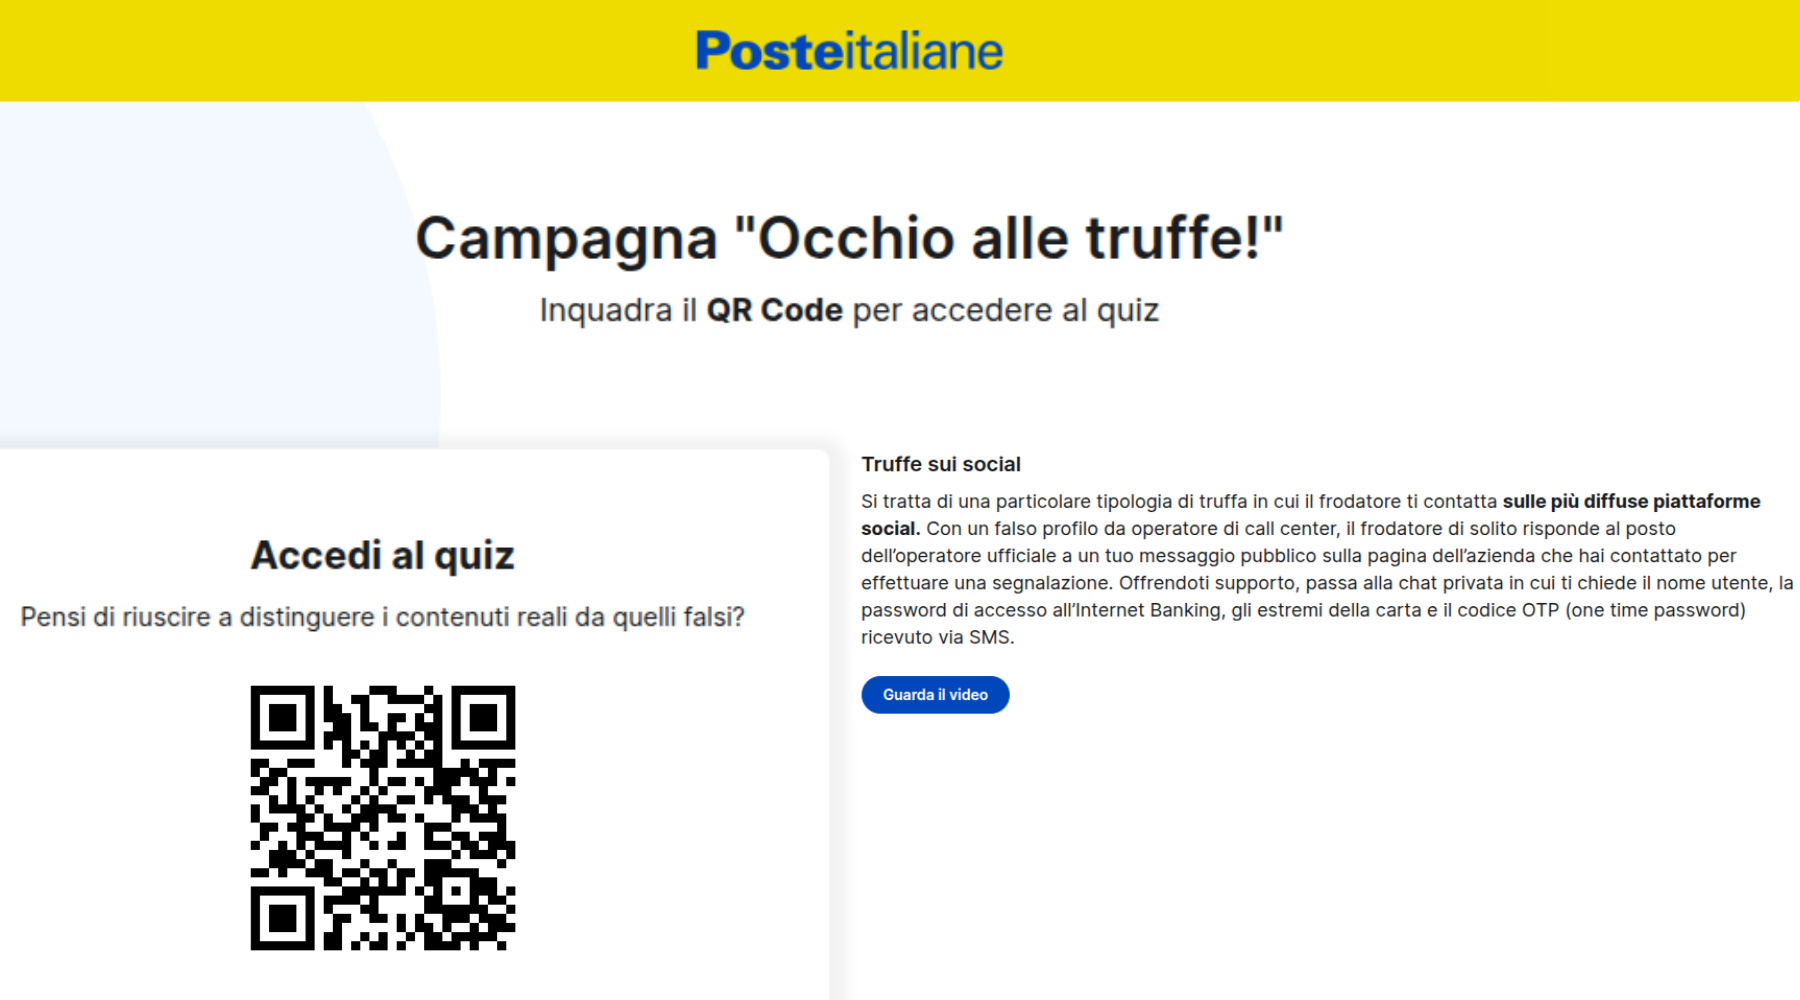
\includegraphics[width=\linewidth]{img/spoofing.png}}
                \caption{{Fonte \href{https://www.poste.it/sicurezza-online/guide-per-operare-in-sicurezza/come-difendersi-dalle-truffe/}{Posteitaliane}}}
            \end{figure}
    \end{columns}
\end{frame}

\begin{frame}{SPOOFING - ESEMPIO}
    \begin{itemize}
        \item \textbf{E-mail spoofing}: l'attaccante (\textbf{Spoofer}) maschera l'indirizzo del mittente di un'email 
        utilizzando software specifico o creando mail che differiscono da quella originale per 
        pochi caratteri simili.
        \pause
        \item \textbf{Spoofing ID chiamante o SMS}: l'attaccante modifica il modo in cui appare il suo 
        numero alle vittime contattate, così che a queste sembri che la chiamata provenga da un numero 
        conosciuto (per esempio quello ``ufficiale'' della banca)
        \pause
        \item \textbf{Web spoofing}: l'attaccante può creare un sito Web falso che 
        sembra del tutto simile a quello utilizzato da una certa azienda.
        \pause
        \item \textbf{IP spoofing}: l'attaccante modifica l'indirizzo IP di origine di un pacchetto o 
        cela l'identità di un dispositivo facendo credere di avere un altro indirizzo IP. 
    \end{itemize}
    \tiny{\textbf{Curiosità}}\\
    \tiny{\href{https://www.geopop.it/una-lettera-contenente-un-qr-code-puo-svuotarvi-il-conto-come-riconoscere-la-truffa-del-postino/}{Truffa del postino}}
\end{frame}

\begin{frame}{PHISHING}
    \begin{alertblock}{DEFINIZIONE}
        \begin{minipage}{0.98\linewidth}
            \justifying
            Il phishing (variante di fishing, ``\textbf{pescare}'') è un tipo di attacco informatico effettuato principalmente tramite \textbf{email}, 
            che ha l'obiettivo di farsi fornire dalla vittima dati personali o finanziari fingendo che 
            l'email provenga da enti come banche, corrieri, piattaforme di streaming o di shopping online. 
            Le email di phishing contengono \textbf{link} che, se cliccati, mettono la vittima a rischio di scaricare 
            \textbf{malware} o consegnare nelle mani del truffatore dati sensibili, come utenze e password, dati bancari 
            e personali.\\
            \bigskip
            \tiny{\textbf{Quiz}}\\
            \tiny{\href{https://phishingquiz.withgoogle.com/}{Sei in grado di riconoscere i tentativi di phishing?}}
        \end{minipage}
    \end{alertblock}
\end{frame}

\begin{frame}{PHISHING}
    \begin{figure}
        \href{https://www.geopop.it/la-truffa-delle-email-cose-il-phishing-e-come-evitarlo/}{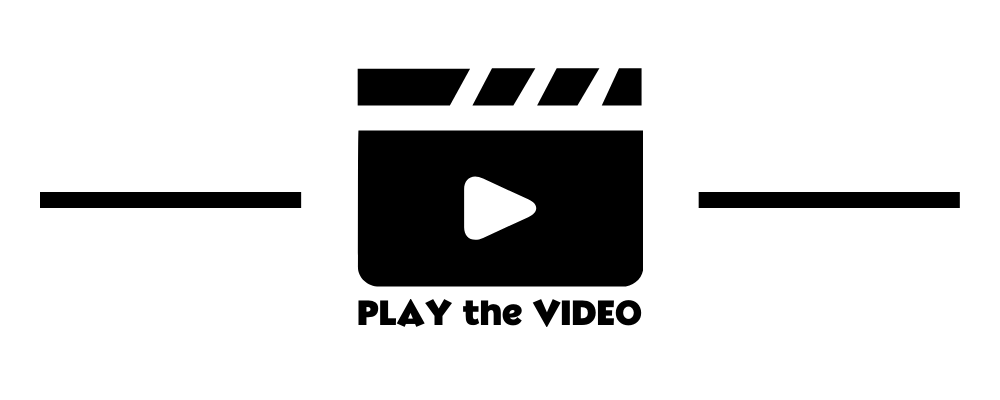
\includegraphics[width=\linewidth]{img/play.png}}
        \caption{{Fonte \href{https://www.geopop.it/la-truffa-delle-email-cose-il-phishing-e-come-evitarlo/}{Come riconoscere un’email di phishing e prevenire la truffa (Geopop)}}}
    \end{figure}   
    \bigskip
    \tiny{\textbf{Curiosità}}\\
    \tiny{\href{https://getgophish.com/}{Open-Source Phishing Framework}}      
\end{frame}

\begin{frame}{SOCIAL ENGINEERING}
    \begin{alertblock}{DEFINIZIONE}
        \begin{minipage}{0.98\linewidth}
            \justifying
            Il \textbf{social engineering} (ingegneria sociale) è una tecnica di manipolazione che \textbf{fa leva sull'errore umano} 
            per ottenere informazioni private, credenziali di accesso o dati di valore. Nell'ambito del 
            cybercrimine, queste truffe basate sullo ``\textbf{human hacking}'' tendono ad adescare gli ignari 
            utenti inducendoli a esporre dati riservati, diffondere infezioni malware o concedere l'accesso 
            a sistemi soggetti a restrizioni. Gli attacchi possono avvenire online, di persona o attraverso 
            altre interazioni.\\
            \bigskip
            \tiny{\textbf{Curiosità}}\\
            \tiny{\href{https://haveibeenpwned.com/}{Check if your email address is in a data breach}}
        \end{minipage}
    \end{alertblock}
\end{frame}

\begin{frame}{SOCIAL ENGINEERING - FASI DELL'ATTACCO}
    \begin{enumerate}
        \item \textbf{PREPARAZIONE}: l'attaccante raccoglie informazioni di carattere generale sulla vittima 
        o su un gruppo più ampio a cui appartiene.
        \pause
        \item \textbf{INFILTRAZIONE}: l'attaccante stabilisce una relazione o da inizio a un'interazione, 
        avviata conquistando la fiducia della vittima.
        \pause
        \item \textbf{SFRUTTAMENTO DELLA VITTIMA}: l'attaccante, dopo aver conquistato la fiducia della vittima 
        e aver identificato un punto debole per sferrare l'attacco, sfrutta la vittima per effettuare il proprio attacco.
        \pause
        \item \textbf{INTERRUZIONE DEI CONTATTI}: l'attaccante infine interrompe i contatti dopo che la vittima ha compiuto l'azione desiderata.
    \end{enumerate}
\end{frame}

\begin{frame}{SOCIAL ENGINEERING - CARATTERISTICHE}
    Gli attacchi di social engineering si basano sul ricorso alla persuasione e alla fiducia da parte 
    dell'attaccante. Quando l'utente è vittima di queste tattiche, è maggiormente incline a effettuare 
    azioni che altrimenti non compierebbe. Tra i tanti tipi di attacchi, la vittima potrebbe lasciarsi fuorviare dai 
    seguenti comportamenti:
    \begin{itemize}
        \item \textbf{EMOZIONI ESASPERATE}: Paura, eccitazione, curiosità, rabbia, senso di colpa, tristezza.
        \pause
        \item \textbf{URGENZA}: La vittima potrebbe essere indotta a compromettersi con il pretesto di un problema 
        serio che richiede attenzione immediata.
        \pause
        \item \textbf{FIDUCIA}: La credibilità è inestimabile ed essenziale in un attacco di social engineering. 
        Dal momento che l'autore dell'attacco sta essenzialmente mentendo, la fiducia gioca un ruolo di primo piano.
    \end{itemize}
    \tiny{\textbf{Curiosità}}\\
    \tiny{\href{https://it.wikipedia.org/wiki/Kevin_Mitnick}{L'hacker più famoso della storia}}
\end{frame}

\section{MALWARE}

\begin{frame}{RABBIT}
    \begin{alertblock}{DEFINIZIONE}
        \begin{minipage}{0.98\linewidth}
            \justifying
            Tipo di malware che \textbf{attacca le risorse del sistema} duplicando in continuazione la propria 
            immagine su disco, o attivando nuovi processi a partire dal proprio eseguibile, 
            in modo da \textbf{consumare tutte le risorse disponibili} sul sistema in pochissimo tempo. 
            Il nome si riferisce proprio alla prolificità di questo "infestante".\\
            \bigskip
            \tiny{\textbf{Esempio}}\\
            \tiny{\href{https://it.wikipedia.org/wiki/Fork_bomb}{Fork Bomb}}
        \end{minipage}
    \end{alertblock}
\end{frame}

\begin{frame}{RABBIT - ESEMPIO FORK BOMB}
    \begin{enumerate}
        \item Creare un file di testo RABBIT.txt;
        \pause
        \item Inserire la Fork Bomb nel file digitando: \textbf{start cmd /k echo BOMB \textbf{$\mid$} \%0}
        \pause
        \item Modificare l’estensione del file da .txt a .bat
        \pause
        \item Preparare un teminale con l'istruzione: \textbf{taskkill /F /IM cmd.exe} per stoppare il malware;
        \pause
        \item Eseguire il file RABBIT.bat e terminarlo con il comando preparato sul terminale.
    \end{enumerate}                        
\end{frame}

\begin{frame}{EFFETTUA UNA RICERCA SUI SEGUENTI MALWARE\\(definizione e un esempio per ogni tipologia)}
    \begin{itemize}
        \item \textbf{BACKDOOR};
        \item \textbf{RANSOMWARE};
        \item \textbf{TROJAN};
        \item \textbf{VIRUS};
        \item \textbf{WORM}.
    \end{itemize}                        
\end{frame}

\begin{frame}{Prof. Eugene Howard Spafford (Spaf)}
    \begin{minipage}{0.98\linewidth}
        \centering
        \huge
        \textit{``L’unico vero sistema sicuro è un sistema spento, chiuso in una gettata di cemento, 
        sigillato in una stanza rivestita di piombo protetta da guardie armate. 
        Ma anche in questo caso ho i miei dubbi.''}
    \end{minipage}
\end{frame}
\end{document}